\documentclass{sigchi}

% Use this command to override the default ACM copyright statement (e.g. for preprints). 
% Consult the conference website for the camera-ready copyright statement.


%% EXAMPLE BEGIN -- HOW TO OVERRIDE THE DEFAULT COPYRIGHT STRIP -- (July 22, 2013 - Paul Baumann)
% \toappear{Permission to make digital or hard copies of all or part of this work for personal or classroom use is 	granted without fee provided that copies are not made or distributed for profit or commercial advantage and that copies bear this notice and the full citation on the first page. Copyrights for components of this work owned by others than ACM must be honored. Abstracting with credit is permitted. To copy otherwise, or republish, to post on servers or to redistribute to lists, requires prior specific permission and/or a fee. Request permissions from permissions@acm.org. \\
% {\emph{CHI'14}}, April 26--May 1, 2014, Toronto, Canada. \\
% Copyright \copyright~2014 ACM ISBN/14/04...\$15.00. \\
% DOI string from ACM form confirmation}
%% EXAMPLE END -- HOW TO OVERRIDE THE DEFAULT COPYRIGHT STRIP -- (July 22, 2013 - Paul Baumann)


% Arabic page numbers for submission. 
% Remove this line to eliminate page numbers for the camera ready copy
% \pagenumbering{arabic}


% Load basic packages
\usepackage{balance}  % to better equalize the last page
\usepackage{graphics} % for EPS, load graphicx instead
\usepackage{times}    % comment if you want LaTeX's default font
\usepackage{url}      % llt: nicely formatted URLs

% llt: Define a global style for URLs, rather that the default one
\makeatletter
\def\url@leostyle{%
  \@ifundefined{selectfont}{\def\UrlFont{\sf}}{\def\UrlFont{\small\bf\ttfamily}}}
\makeatother
\urlstyle{leo}


% To make various LaTeX processors do the right thing with page size.
\def\pprw{8.5in}
\def\pprh{11in}
\special{papersize=\pprw,\pprh}
\setlength{\paperwidth}{\pprw}
\setlength{\paperheight}{\pprh}
\setlength{\pdfpagewidth}{\pprw}
\setlength{\pdfpageheight}{\pprh}

% Make sure hyperref comes last of your loaded packages, 
% to give it a fighting chance of not being over-written, 
% since its job is to redefine many LaTeX commands.
\usepackage[pdftex]{hyperref}
\hypersetup{
pdftitle={SIGCHI Conference Proceedings Format},
pdfauthor={LaTeX},
pdfkeywords={SIGCHI, proceedings, archival format},
bookmarksnumbered,
pdfstartview={FitH},
colorlinks,
citecolor=black,
filecolor=black,
linkcolor=black,
urlcolor=black,
breaklinks=true,
}

% create a shortcut to typeset table headings
\newcommand\tabhead[1]{\small\textbf{#1}}


% End of preamble. Here it comes the document.
\begin{document}

\title{Brain Speed Reader: A Neurofeedback Apparatus to Read Fast and Remediate Multi-tasking.}

\numberofauthors{1}
\author{
  \alignauthor Anonymous Authors\\
    \affaddr{Anonymous Affiliations}\\
    }


%\numberofauthors{4}
%\author{
%  \alignauthor 1st Author Name\\
%    \affaddr{Affiliation}\\
%    \affaddr{Address}\\
%    \email{e-mail address}\\
%    \affaddr{Optional phone number}
%  \alignauthor 2nd Author Name\\
%    \affaddr{Affiliation}\\
%    \affaddr{Address}\\
%    \email{e-mail address}\\
%    \affaddr{Optional phone number}    
%  \alignauthor 3rd Author Name\\
%    \affaddr{Affiliation}\\
%    \affaddr{Address}\\
%    \email{e-mail address}\\
%    \affaddr{Optional phone number}
%      \alignauthor 4th Author Name\\
%    \affaddr{Affiliation}\\
%    \affaddr{Address}\\
%    \email{e-mail address}\\
%    \affaddr{Optional phone number}
%}
%
\maketitle

\begin{abstract}
At the age of online information abundance, the human capacity to retain knowledge is largely limited by the time and the attention required to read text, watch videos, listen to podcasts. For written information, rapid serial visual presentation (RSVP) helps greatly save time with similar levels of text understanding, compared with traditional reading. However, RSVP does not account for attention. We present a simple hybrid brain-computer interface (BCI) that controls in real-time the speed of reading by measuring the instant level of higher cognitive brain activity. Electroencephalogram (EEG) signal is acquired with a single channel consumer-grade headset and analyzed in the frequency domain. The pace of word display is controlled by a measure brainwave entropy. We have conducted a controlled experiment with 50 subjects with three distinct treatments, and we show that brain-controlled speed-reading increases the speed and the understanding of texts by subjects.
\end{abstract}

\section{Introduction}
\section{Background}
\label{background}

\subsection{Rapid serial visual presentation}
In the same way as we do here, but for different purpose, researchers in cognitive science have long been interested in pushing the limits of human brain capabilities. Designing experiments that way has helped understanding neuro-cognitive processes associated with e.g., information processing, memory mechanisms, and concentration. One way of pushing the limits is by exposing individuals to a fast paced sequence of stimuli with a tachistoscope. The first tachistoscope was originally described by the German physiologist A.W. Volkmann in 1859 as device that displays an image for a short amount of time using a specific mechanical shutter \cite{benschop1998tachistoscope}. The tachistoscope found a practical application  during World War II in the training of fighter pilots to help them identify aircraft silhouettes as friend or foe \cite{godnig2003tachistoscope}. With text presented (instead of images), the tachistoscope was subsequently used in the late fifties and sixties, in school for the purpose of teaching reading and to help improve reading comprehension \cite{brown1958teaching}, as well as in cognitive sciences for the purpose of rapid serial visual presentation (RSVP) \cite{potter1984rapid,potter1975time}. RSVP helped gain insights on cognitive mechanisms associated with language processing \cite{potter1984rapid}, short- and long-term memory as well as conceptual memory \cite{potter1993very}, the attentional blink \cite{shapiro1994attention}, comprehension \cite{weiss2005increased} and multi-tasking \cite{jolicoeur200013}. Nowadays, the tachistoscope has been replaced by computer screens, and RSVP is still a dominant technique to test research paradigms in cognitive neuroscience in particular in relation with language. Rapid serial visual presentation is most often coupled with neuro-imaging devices, such as electroencephalograms \cite{kranczioch2006eeg,mathan2008rapid}, and fMRI (dual-tasking)\cite{marcantoni2003neural}. 

Rapid serial visual presentation has also been found to be useful to enhance reading speed for individuals, in particular for people suffering from reading impairments. For instance, Chen (1983) found that the half of his college subjects who were less good readers remember more from RSVP paragraphs than from conventional paragraphs viewed for the same total time; the better readers showed a slight but not significant drop, with RSVP \cite{chen1986effects}. Similarly, scrolled and rapid serial visual presentation texts are read at similar rates by the visually impaired \cite{fine1995scrolled}.

\subsection{Brain computer interfaces, control \& consumer markets}
Rapid serial visual presentation is not a brain-computer interface (BCI) because, the brain of the individual exposed to the fast-paced sequence of stimuli has no control on the sequence itself. On the contrary, brain-computer interfaces enable a direct communication between computers and brains, usually through the signal processing of evoked response potentials \cite{vidal1973toward}. Research on BCI spans from restoring capabilities for heavily motor-impaired disabled \cite{galan2008brain}, to the rehabilitation and training  \cite{daly2008brain} of focused cognitive capabilities, to consumer market applications, including e.g., computer passwords encoded as {\it passthoughts} as a form of two-factor authentication relying on a mental gesture combined with inner biological brain signal \cite{chuang2013ithink,jonhson2014mythoughts}, mental tasks classifiers \cite{merrill2015}, or drowsiness detectors for drivers \cite{liu2013driverAlertness}. EEG technology used for BCIs ranges from \$100 consumer grade devices as the one used here, to micro electrodes implanted in the brain as used to control the simulation of steering a fighter jet \cite{BCIfighterJet2015}.

\subsection{Neurofeedback \& self-regulation}
One of the most used brain computer control mechanism is neurofeedback. From early research on operational conditioning of cats \cite{wyrwicka1968instrumental,sterman1969electrophysiological}, neurofeedback has been found to ``train the brain" in order to remediate brain disorders, such as for attention deficit hyperactivity disorder \cite{lubar1976eeg,monastra2006electroencephalographic},  depression \cite{saxby1995alpha},  post-traumatic syndrom disorder \cite{peniston1991alpha}, or autism \cite{kouijzer2009neurofeedback,coben2010neurofeedback}, to reduce the incidence of epileptic seizures \cite{sterman2006foundation}. Neurofeedback is also thought to enhance cognitive performance, namely for music \cite{egner2003ecological}, sport \cite{wilson2006mind}, control of emotions \cite{gruzelier2014eeg} and mood \cite{raymond2005effects}, or to help the practice of meditation \cite{gruzelier2009theory,rubik2011neurofeedback,brandmeyer2013meditation}. Because the mechanisms of neurofeedback remain unclear, the validity of theories and results remain questioned \cite{beyerstein1990brainscams,vernon2009alpha}.

Most studies consider brain activity as a variable dependent of exogenous stimulations  (e.g., visual or auditory stimuli) and measure brain response and adaptation to these well calibrated stimuli (resp. behaviors), with focus on electroencephalogram (EEG) frequency bands, such as increase the sensorimotor rhythm (SMR, 12-14 Hz band), alpha band (7.5 - 12.5 Hz), beta band (15 - 20 Hz) , theta band (6-10 Hz), gamma band (25 -100 Hz), and a multitude increased / decreased band activity combinations. However, these frequency bands and their activations are individual specific, and are dependent to a number of factors, including age \cite{} and cognition training following exposure to stimuli \cite{}. As a method intended to train specific frequency bands (i.e., change their intensity following stimuli or behaviors), neurofeedback embodies this plasticity, but it generally assumes that frequency bands are invariant across subjects. Therefore, most experiments target and train pre-determined frequency bands. 

In contrast, neurofeedback experiments can also use self-regulated brain activity to study voluntary controlled behaviors, and conversely, the nature of brain activity can be unveiled from observed behaviors. Functional magnetic resonance imaging (fMRI) is a powerful tool for source localization, and methods have been developed recently for real-time fMRI (rtfMRI), which allow exposing subjects to brain triggered stimuli (audio or video) and at the same time map brain activity \cite{}. Feedback obtained from rtfMRI is slow however (between 1 and 2 seconds) as fMRI measures the blood oxygenation level dependent signal \cite{ogawa1990brain,ogawa1990oxygenation}. Feedback speed may also be an issue with EEG, depending on the amount of required signal processing (e.g., artifact removal, blind source separation), which is highly dependent on the quality of the equipment used and the desired resolution, in particular for source localization.

%The varied yet repeated patterns observed in the brain has provided hope for applications relying on a direct interface between the brain, a processing unit (e.g., a computer), and by extension any system controlled by a computer. Applications involving brain computer interfaces (BCI) span from neurological rehabilitation \cite{daly2008brain} to neurofeedback \cite{lubar1995evaluation,fuchs2003neurofeedback} to brain-controlled wheelchairs \cite{galan2008brain}, or even steering a fighter jet simulation with a robotic arm controlled through 96 micro electrodes implanted in the brain \cite{BCIfighterJet2015}.

%Most current BCI approaches are developed in the lab, and most often for very specific applications involving rehabilitation and remediation, mainly building on the temporal characteristics of the EEG signal, namely event-related potential (ERP) \cite{brouwer2010tactile}. Recent work has however featured results obtained with consumer grade EEG headsets, which price is of the order of a few hundred dollars. For instance, it has been demonstrated that the signal of a Neurosky Mindset, a single channel dry EEG headset, can be used to improve driver alertness through appropriate music selection, through a drowsiness detector, involving a combination of machine learning techniques \cite{liu2013driverAlertness}. The same Neurosky device may help bring ``passthoughts"  to the consumer market, as a form of two-factor authentication relying on a mental gesture combined with inner biological brain signal \cite{chuang2013ithink}. This passtought approach has recently been further tested and found to be robust against impersonation attacks \cite{jonhson2014mythoughts}. Building on the same approach, Merrill et al. \cite{merrill2015} developed a simple approach for the classification of mental tasks, using logarithmic quantization combined with a progressive calibration technique. Overall, comparison of consumer-grade single channel EEG with research-grade EEG shows that while consumer-grade EEG cannot locate the origin of the signal, it can discriminate well enough variations of power spectrum intensity, and thus, has potential utility for tasks requiring portability and ease of use \cite{johnstone2012eeg}.


%\subsection{(optional) Language \& neurosciences}
%Language is intimately related to cognitive processes associated with memory, and because it is a feature almost unique human beings, it accounts as one of the most interesting, challenging and highly investigated research topics in neuroscience \cite{beeman1998right,pulvermuller2002neuroscience}. Language has traditionally been attributed to the Broca Region {\bf [say more here from the paper]} \cite{keller2009broca} and, it was found that left prefrontal brain regions are substantially more involved during encoding of verbal stimuli, which is correlated with increased involvement of the semantic memory system and simultaneous encoding into the short-term memory \cite{fletcher1998functiona,tulving1994hemispheric}. Language processing being a complex task, not only one region and particular frequency ranges of the brain are involved. Weiss et al. \cite{weiss2000long} found long-range EEG synchronization during word encoding associated with high memory performance (primarily between the prefrontal and temporal-parietal regions), as well as an increase in spectral activity in the lower frequencies \cite{kujala2007phase}. It was also found that higher frequencies (Gamma range $>20Hz$) exhibit an increased intensity during processing of words \cite{pulvermuller1995spectral}. From EEG studies, it was found that language processing triggers increased neuronal communication in a variety of regions, but importantly in the frontal-parietal region, and over many frequency ranges [$\theta$ (4 to 7 Hz),$\beta_1$ (13 to 18 Hz) and $\gamma$ (30 to 34 Hz)] \cite{weiss2005increased}. A recent RSVP study combined with Magnetoencephalogram (MEG) spatio-temporal acquisition of coherence of brain regions brought evidence that the 8-13 Hz frequency range (followed by 16-24Hz for four over nine subjects) accounts for most signal associated with reading, and across brain regions, with particularly high coherence density {\bf [explain or rephrase this]} in the frontal-parietal region \cite{kujala2007phase}, although a number of other regions appear to be involved with the cognition processed associated with language processing and reading, reflecting the necessary complex cognitive operations associated with a complex interplay of neuronal synchronizations in the spatial and frequency domains.




%For example, a short time latency after a sentence or paragraph usually improves knowledge integration \cite{see review by potter}. Also, the time required to reading a series of words in natural language can be estimated at the word level as being logarithmic of the word predictability, which is itself related to word congruence in the text \cite{smith2013effect}. \textcolor{red}{\bf [I am still missing some references on the processing lag (between stimulus and conceptualization ($~200ms$?]}

%\subsection{Neurosciences of Natural Language Processing}
%With the development of neuroimaging techniques, such as electroencephalograms (EEG), magnetic resonance imaging (MRI), and functional MRI (fMRI), the study of cognitive processes has become physiological, with improved possibilities to observe brain activations in space and time, following one or multiple stimuli. For instance, neuroimaging of short-term and long-term memory processes has been studied with EEG in the spectral dimension \cite{klimesch1999eeg,khader2011eeg}, and suggest that increased activity within the upper alpha () and theta () frequency bands correlate with search and retrieval processes of semantic information stored in cortical associative networks \cite{klimesch1996memory,klimesch1990alpha}. Results from several studies \cite{khader2011eeg} suggest that upper alpha seems to be related to semantic long-term memory (LTM) retrieval, while theta activity seems to be related to episodic LTM encoding \cite{} and the maintenance of information in short-term working memory \cite{}. 

%EEG alpha and theta oscillations reflect cognitive and memory performance: a review and analysis \cite{klimesch1999eeg}, as well as in relation with short-term and long-term memories.  \cite{khader2011eeg}. 



%(MRI study?) Activation of left prefrontal and medial temporal cortices were engaged during the encoding of both recalled and forgotten words \cite{wagner1998building}. At least partially supported by Kapur et al. \cite{kapur1996neural} in a PET (positron emission tomography) study 

%Processing new and repeated names: Effects of coreference on repetition priming with speech and fast RSVP  (ERP?) \cite{camblin2007processing}

%o our knowledge, nothing has been done related to language with consumer grade EEG.
%Here, we shall show that existing research work supports the hypothesis that a single EEG channel set on the forehead, can detect useful signal for our purpose, and show that we do is feasible, at least in principle. {\bf [Important parameters : main location of signal, wave frequency, and maybe latency]}. 



%We are aware that our input device is of low quality, and cannot, by design, capture spatial brain activation (there is only one electrode). Also, we assume that the low quality (i.e., one channel with dry EEG) is not sufficient to capture time delays (ERPs), usually observed in response to stimuli \cite{}. 

%\subsection{RSVP, Cognition and Memory}
%Research on cognition relating to a rapid sequence of words \cite{forster1970visual} and pictures \cite{potter1975time,potter1969recognition} go back to the 70's and 80's. RSVP offers a way to control these processes at fine-grained level. Rapid serial visual presentation (RSVP): A method for studying language processing \cite{potter1984rapid} 
%
%
%This research is centered on (i) how long it takes to internalize the meaning of a word or a sentence, sufficiently that it is possible to recall it accurately, (ii) what kinds of memory processes are solicited [short-term memory (STM) or iconic memory, long-term memory (LTM), working memory (WM)], and (iii) how these are engaged to transform ``raw" information into ``conceptual" information, which can be recalled more easy \cite{}. To emphasize on the interplay between STM bringing information, and LTM pulling out useful concepts for broader understanding, Molly Potter introduced Conceptual Short-Term Memory (CSTM) \cite{potter1993very}. ``Unlike STM, CSTM is central to cognitive processing.
%Recognition of meaningful stimuli such as words or objects
%rapidly activates conceptual information and leads
%to the retrieval of additional relevant information from
%LTM." \cite{potter1993very}. It also depends on the goals set: e.g., identify a specific item in a list, or get a conceptual understanding of a sequence.

%It is important to point out the difference between the capacity to recall unrelated words versus semantically related words, but also, in the case of whole paragraphs, some (short) time is required after a sentence to integrate knowledge \cite{}.



%Visual perception of rapidly presented word sequences of varying complexity 

%Temporal limits of selection and memory encoding a comparison of whole versus partial report in rapid serial visual presentation \cite{nieuwenstein2006temporal}

%Rapid serial visual presentation: a space-time trade-off in information presentation \cite{de2000rapid}

%\subsection{Memory and Time to Process Information}
%``When people view or listen to continuous sequences of scenes or
%words, as they do when they look around, read, listen, or watch TV,
%a series of conceptual representations is activated. These rapidly activated
%and equally rapidly forgotten representations are the raw material
%for identification and comprehension of words, pictures, and
%sequences such as a sentence, and indeed for intelligent thought more
%generally. The normal ease with which we understand what we read
%and see around us is based on selective processing that takes place
%much faster than has been supposed in many theories of working and
%short-term memory, leading to the CSTM hypothesis." \cite{potter1999understanding,potter1993very}
%
%``CSTM is a processing and memory system different from early visual (iconic)
%memory, conventional short-term memory (STM), and longer-term
%memory (LTh{) in three important respects: (1) the rapidity with which
%stimuli readr a postcategoricaf meaningful level of representation, (2)
%the rapid struchrring of these representations, and (3) the lack of awareness
%(or immediate forgetting) of inforrration that is not structured
%or otherwise consolidated. Structure-building in CSTM ranges from
%spontaneous grouping of words in lists on the basis of meaning (one
%of the simplest forrrs of conceptual structuring) to linguistic parsing
%and semantic interpretation of sentences and more extended texts
%(examples of highly skilled structuring). Organization or structuring
%of new stimuli enhances memory for them." \cite{potter1999understanding}
%
%A capacity theory of comprehension: individual differences in working memory \cite{just1992capacity}
%
%Individual differences in working memory and reading \cite{daneman1980individual}
%
%``Second, this information is used in various ways, depending on the
%viewer's current goal if the viewer is trying to understand the whole
%sequence (e.9., a sentence), the information is used to discover or build
%a comprehensive structured representation, but if the viewer is trying
%to locate and identify a particular kind of information (as in target
%search), then only a subset of the information is selected." \cite{potter1999understanding}
%
%``processingT. he CSTM hypothesis
%is not only that conceptual information is activated rapidly, but
%also that the initial activation is highly unstable, such that the
%information is deactivated or forgotten within a few hundred
%msec if it is not incorporated into a structure (or selected for
%further processing" \cite{potter1999understanding}
%














\section{Method}

\subsection{Brain Speed Reader}

{\bf describe the brain control system}

\begin{enumerate}
  \item capture brainwaves for 1 second
  \item compute power spectrum
  \item compute normalized entropy
  \item update display speed ({\bf trick of the moving average to be described here})
\end{enumerate}


\subsection{Experimental Protocol}


\begin{enumerate}
  \item Constant Rate
  %\item Randomly Varying Text : AR(1) $\rigtharrow$ AR1(n,baseline,baseline/2,0.5,sigma=std) AR1 formula : $c + phi * X[-1] + np.random.normal(scale=sigma)$
  %\item Brain Speed Reader : (i) compute entropy $S$ at t, (ii) normalize $S$ as $S_{norm} = (S- \langle S \rangle) / \sigma_S$, with $\langle S \rangle$ and $\sigma_S$ computed over the last XX values of entropy, (iii) compute a new speed as $v(t+1) = v(t)\cdot(1-0.2\sdot S_{norm})$
\end{enumerate}


\subsection{Measuring Text Complexity}

ATOS  ( ref: Michael Milone,The Development of ATOS, The Renaissance Readability Formula, p10 (2010) \url{http://doc.renlearn.com/KMNet/R004250827GJ11C4.pdf}

\begin{itemize}
  \item Words per sentence
  \item Average grade level of words ( which class grade the word is first seen)
  \item Characters per word
\end{itemize}


$ATOS Rasch Difficulty Formula = -8.54 + 1.95 * Ln(AvgWords) + .46 * AvgGrad100 + 1.74 * Ln(AvgChar)$

Adjustment for books with less than 500 words

$BLGL for Books With Fewer Than 500 Words = .004 * Book Length + 0.4$


Table detailing texts : \url{https://docs.google.com/spreadsheets/d/1uwkoToM-p3UFrd0U_1vOX4eBJsmYuPVYVhvhsZ8Y5Nc/edit#gid=0}




%\begin{itemize}
%  \item {\bf text 0 (adapted from Coming of Age in Samoa, Margaret Mead, 1928
%)}:   $ATOS=9.5$,  $word~count = 421$
%  \item {\bf Text 1  (adapted from The Warden, Anthony Trollope, 1855)} : $ATOS=8.3$, $word~count = 563$
%  \item {\bf Text 2  (adapted from The Mayor of Casterbridge, Thomas Hardy, 1886) } : $ATOS=10.2$, $word~count = 831$
%  \item {\bf Text 3 (Adapted from: The Social Function of Science, John D Bernal (1939))} : $ATOS=11.9$, $word~count = 421$
%\end{itemize}



\section{Experimental Protocol}
To determine the gains of our brain speed-reader apparatus when reading, we have conducted an experiment, involving XX subjects who participated in our study. The experimental procedures described here were approved by an Institutional Review Board. 

\subsection{Procedure}
After obtaining individual consent, we conducted a quick {\bf calibration} task. A text was displayed word by word to each subject, who could adapt the rate of word display with the right (faster) and left (slower) arrow keys, until they reach their comfort zone. This baseline rate would be reused during the experiment. Then, the subject was asked to {\bf wear} the Neurosky Mindset. When ready, a {\bf text was displayed word by word} in a Rapid Visual Serial Presentation (RVSP) manner. After all text was been displayed, the subject was asked some comprehension questions regarding the content of the text. This procedure was repeated three or four times with various texts and various treatments involving varying the rate $R$ of word display:

\begin{enumerate}
  \item {\bf Constant Rate: } the rate of word display remains constant with $R(t) = R_{0}$ for $\forall t$.  
  \item {\bf Brainwave Treatment: } starting from the baseline $R_0$, the rate $R$ changes every quarter second as a function of the rate at the previous step and as a function of the entropy $S_{norm}$ measured in real-time from the EEG captured by the Neurosky mindset, and according to formula (\ref{eq:RateChange}).
    \item {\bf Random Rate Treatment: }  %Randomly Varying Text : R(1) $\rigtharrow$ AR1(n,baseline,baseline/2,0.5,sigma=std) AR1 formula : c + phi * X[-1] + np.random.normal(scale=sigma)
\end{enumerate}

The subject was wearing the Neurosky headset and was not informed whether the treatment involved using EEG as an input for controlling the rate $R$ of word display. In other word, the subject and no information on the three treatments, and had no possibility to distinguish between these treatments, in other ways than guessing from their experience.

In case, four treatments were applied, one of the treatments was repeated once with a different text. After the end, subjects were asked to fill short surveys for each text, asking about comfort, perceived level of understanding, degree of control, followed by a survey to collect demographic informations.

\subsection{Measuring Text Complexity}

ATOS  ( ref: Michael Milone,The Development of ATOS, The Renaissance Readability Formula, p10 (2010) \url{http://doc.renlearn.com/KMNet/R004250827GJ11C4.pdf}

\begin{itemize}
  \item Words per sentence
  \item Average grade level of words ( which class grade the word is first seen)
  \item Characters per word
\end{itemize}


$ATOS Rasch Difficulty Formula = -8.54 + 1.95 * Ln(AvgWords) + .46 * AvgGrad100 + 1.74 * Ln(AvgChar)$

Adjustment for books with less than 500 words

$BLGL for Books With Fewer Than 500 Words = .004 * Book Length + 0.4$


Table detailing texts : \url{https://docs.google.com/spreadsheets/d/1uwkoToM-p3UFrd0U_1vOX4eBJsmYuPVYVhvhsZ8Y5Nc/edit#gid=0}




%\begin{itemize}
%  \item {\bf text 0 (adapted from Coming of Age in Samoa, Margaret Mead, 1928
%)}:   $ATOS=9.5$,  $word~count = 421$
%  \item {\bf Text 1  (adapted from The Warden, Anthony Trollope, 1855)} : $ATOS=8.3$, $word~count = 563$
%  \item {\bf Text 2  (adapted from The Mayor of Casterbridge, Thomas Hardy, 1886) } : $ATOS=10.2$, $word~count = 831$
%  \item {\bf Text 3 (Adapted from: The Social Function of Science, John D Bernal (1939))} : $ATOS=11.9$, $word~count = 421$
%\end{itemize}



\section{Results}
\label{results}


For $17$ over $21$ participants, the RSVP rate was characterized by a balanced joint probability of {\it rate change x word size frequency} in treatment (ii) and (iii) (Fig. 2a). Long words triggered the largest change of entropy (resp. rate), while words smaller than the average size ( $< 5.5$ characters) were associated with reverse entropy (resp. rate) change (Fig. 2b, 2c).\\

Despite the large variation of entropy, texts could be decoded by matching the sequence of entropy measures (associated with each word) with the unique sequence of word lengths (Fig 3). Our results did not require preliminary identification of participants, and the success rate was 27.4\%, roughly 11\% above chance (i.e., $1/6 \approx 16.67\%$), when considering the first 300 words of each text.



\begin{itemize}
  \item performance*, perceived comfort and control as a function of treatment 
  \item for brain speed reader treatment:  performance*, perceived comfort and control as a function $X_0$, $alpha$
\end{itemize}

*performance means either {\bf conceptual} (understanding the meaning), {\bf conceptual-memory} (recalling characters) or {\bf memory} (recalling some words).



\section{Discussion}
\label{discussion}
Recognizing the importance of reading more in less time, while avoiding multi-tasking, we have put to the test the {\it brain speed reader}, a brain-computer interface (BCI) implementing a rate varying rapid serial visual presentation (RSVP) of text words. We have found that a majority of users who participated in our study could control the brain speed reader. Furthermore, we found that roughly half of participants could self-regulate with two opposite control mechanisms ({\it bsr+} and {\it bsr-}). The achievement of self-regulation is negatively influenced by age, text length, topic familiarity and speed reading comfort. Self-regulation achievement (stability) is however highly positively correlated with reading pleasure. Capacity to provide a meaningful text summary {\it ex-post} (the best way to test for text comprehension) is also positively associated with stability, yet in a weakly significant way.

Our results show that the brain speed reader is an adequate technology to foster fast knowledge integration in a world of abundant information and endless news feeds, while at the same time helping preventing multi-tasking. The design implements self-regulation neurofeedback as a way to ensure that users concentrate on reading the text: If the user does not or cannot concentrate, the RSVP rate will drift towards very slow (resp. fast) word display rates. Multi-tasking is discouraged by design, and reading speed is doubled compared to normal reading.

Self-regulation neurofeedback stems from the capacity by the brain to train and adapt its wave modulations in order to perform specific tasks better \cite{piano_neurofeedback}, or to reach desired mental states \cite{neurofeedback_meditation}.  As a special kind of neurofeedback BCI, the brain speed reader may be help remediate reading disabilities or difficulties associated with a lack of concentration capabilities, which is one consequence of multi-tasking. Because the brain speed reader (BSR) does not require prior calibration, training and use occur concomitantly: Either the user achieves self-regulation quickly and then {\it uses} BSR, or she remains in training mode until she reaches self-regulation. In our experiment, we have set very large boundary for slowest (resp. fastest) RSVP rate to make sure that subjects who reach the boundaries effectively failed achieving self-regulation. In training mode, these RSVP rate boundaries may be tuned and personalized to ensure that the user can reach a compromise between attempts to achieve self-regulation and still reading fast with pleasure while training. While we have not tested medical applications for the brain speed reader, it may help users suffering from dyslexia or attention disorder and hyperactivity disorders (ADHD) improve their reading and their attention.

\subsection{Limitations}
The version of the brain speed reader presented here is a first attempt to harness self-regulated neurofeedback for the sake of upgrading the reading experience to arising challenges in society, such as tackling the abundance of natural language- written information while reducing multi-tasking. Although our first experiment show encouraging results, we have come up with the simplest possible implementation and experimental protocol. A number of outstanding questions remain and deserve further work, starting with the hardware we used. Neurofeedback most often involves a limited number of EEG electrodes, but typically of higher quality and on other positions in the 10-20 system. One may want to experiment with a variety of electrode quality, number, and positions to elicit a better hardware configuration.

Our study bears a number of limitations regarding comprehension and memory. We did not find a significant difference of comprehension between RSVP speed read at constant rate versus {\it bsr+} and {\it bsr-} treatments. We find a slight comprehension improvement when users achieve more stable self-regulation, but this result need further validation, presumably with a larger data set. We have also not measured how comprehension and word recall are diminished (resp. increased) as reading speed doubles, i.e., when comparing brain speed reading and reading text normally. Previous research suggests that comprehension is diminished by constant RSVP rate speed reading \cite{kujala2007phase}, although it remains the same or is slightly improved for people with reading disabilities. Further investigation is required to better elicit how self-regulation stability influences comprehension and word recall

We shall also investigate why some participants could not achieve self-regulation: It remains unclear if they had indeed to train further before making it right, or if the BSR parameters we chose [initial RSVP rate $X(t=0) = 125$ ms/word and $|\alpha| = 0.005$] may only be suitable for a subset of the population, and may require further adaptation. Similarly, we have no information on the time it takes to learn given that the user could not achieve self-regulation at once. We chose $X(t=0) = 125$ ms/word as the starting RSVP rate, which is also the value known to be most comfortable on average to people who read with RSVP. To further understand and validate the self-regulation mechanism, it would be desirable to perform additional investigations with a variety of starting rates. Our hypothesis is that within a yet unknown RSVP rate range, users capable of self-regulation can stabilize the rate, while beyond some limits it is impossible to control the brain speed reader, in particular when the presentation speed is high. It also remains to be seen if users tend to stabilize the rate close to 125ms/word on average, even if the initial RSVP rate is smaller (resp. larger).

Even though there is no need for preliminary {\it ad-hoc} calibration to use the brain speed reader, learning still occurs ``on the fly", with several advantages as already mentioned above. It would nevertheless be desirable to better understand how the user transitions from {\it learning} to {\it using}. This has implications for more elaborate and personalized UX design.

Finally, we found that text length has a negative effect on self-regulation stability (roughly one unit per 1300 words as shown in Table \ref{tab:reg}). This is a concern because the brain speed reader is supposed to let users avoid multi-tasking to concentrate on a single task instead. Here, it appears that if the task lasts too long, then self-regulation undergo changes of regime and reduced stability. This suggests that either BSR is suited for {\it long but not that long tasks} and/or there is another factor involving learning how to keep self-regulation highly stable over long tasks. This is has further implications on comprehension and memory, which need to be further addressed.

\subsection{Beyond speed reading}
Here, we have designed and tested brain-computer interface (BCI), which helps seamlessly control the parsing rate of a coherent sequence of a words as visual stimuli. The same time varying rate RSVP coupled with a neurofeedback BCI may be used beyond reading. It could apply similarly to cartoons, video or audio streams, if the control is made on the continuous speed (i.e., the pitch) of the media stream, similarly to the (discrete) presentation rate used in our experiment.

Similar BCI could be used to assess the quality and the coherence of a piece of text. Indeed, it appears that when reading, the brain makes some heuristic predictions of what word(s) is (resp. are) coming next \cite{smith2013effect}. Unexpected words trigger an unusual cognitive activity which slows the reading. Recording how the effects of unexpected stimuli materialize in conjunction with control remain yet to the be investigated. 


\section{Conclusion}
\label{conclusion}
%Recognizing the importance of reading more in less time, while avoiding multi-tasking, a way to do more in less time, yet most often at the cost of less grasp on tasks at hand

In this article, we have proposed, designed and tested a new approach to brain computer interfaces, geared towards handling and controlling a fast-paced flow of information in way that limits diversion from the focal taks and hence, prevents multi-tasking. Our approach is based on a peculiar and seldom phenomenon occurring in the brain -- known as {\it self-regulation}. This phenomenon can be assimilated to independent neurofeedback. We have then tested and benchmarked the so-called {\it brain speed reader} in the context of reading text, and we have found that a large proportion of participants to our experiment successfully achieved self-regulation without prior training for at least one of both treatments proposed. On average they would read twice as fast as with normal reading. We furthermore found that age, text length and speed reading comfort have a negative effect on the achievement of self-regulation. On the contrary, capacity to read fast in a normal setting, and reading pleasure have a positive impact on stability. The pleasure in reading suggests the existence of a reward mechanism when a participant achieves self-regulation. Comprehension is only weakly improved when self-regulation is achieved. 

%``It would elevate the computer to a genuine prosthetic extension of the brain" (Vidal 1973)
%``(to identify appropriate correlates of mental states and decisions in external signals" (Vidal 1973)




%\keywords{
%	Guides; instructions; author's kit; conference publications;
%	keywords should be separated by a semi-colon. \newline
%	\textcolor{red}{Optional section to be included in your final version, 
%  but strongly encouraged.}
%}
%
%\category{H.5.m.}{Information Interfaces and Presentation (e.g. HCI)}{Miscellaneous}
%
%See: \url{http://www.acm.org/about/class/1998/}
%for more information and the full list of ACM classifiers
%and descriptors. \newline
%\textcolor{red}{Optional section to be included in your final version, 
%but strongly encouraged. On the submission page only the classifiers’ 
%letter-number combination will need to be entered.}
%
%\section{Introduction}
%
%This format is to be used for submissions that are
%published in the conference proceedings.  We wish to give
%this volume a consistent, high-quality appearance. We
%therefore ask that authors follow some simple
%guidelines. In essence, you should format your paper
%exactly like this document. The easiest way to do this is
%simply to download a template from the conference web
%site, and replace the content with your own material.
%
%\section{Page Size and Columns}
%
%On each page your material (not including the page number) should fit
%within a rectangle of 18 x 23.5 cm (7 x 9.25 in.), centered on a US
%letter page, beginning 1.9 cm (.75 in.) from the top of the page, with
%a .85 cm (.33 in.) space between two 8.4 cm (3.3 in.) columns.  Right
%margins should be justified, not ragged. Beware, especially when using
%this template on a Macintosh, Word can change these dimensions in
%unexpected ways. Please be sure that your PDF is US letter and not
%A4. If your PDF or paper are formatted for A4, the submission will be
%returned to you to fix.
%
%\section{Typeset Text}
%
%Prepare your submissions on a word processor or typesetter.  Please
%note that page layout may change slightly depending upon the printer
%you have specified.  \LaTeX\ sometimes will create overfull lines
%that extend into columns.  To attempt to combat this, the .cls
%file has a command, {\textbackslash}sloppy, that essentially asks
%\LaTeX\ to prefer underfull lines with extra whitespace.  For more
%details on this, and info on how to control it more finely, check out
%{\url{http://www.economics.utoronto.ca/osborne/latex/PMAKEUP.HTM}}.
%
%\subsection{Title and Authors}
%
%Your paper's title, authors and affiliations should run across the
%full width of the page in a single column 17.8 cm (7 in.) wide.  The
%title should be in Helvetica 18-point bold; use Arial if Helvetica is
%not available.  Authors' names should be in Times Roman 12-point bold,
%and affiliations in Times Roman 12-point.  For more than three authors,
%you may have to place some address information in a footnote, or in a named
%section at the end of your paper. Please use full international addresses and
%telephone dialing prefixes.  Leave one 10-pt line of white space below the last
%line of affiliations.
%
%\subsection{Abstract and Keywords}
%
%Every submission should begin with an abstract of about 150 words,
%followed by a set of keywords. The abstract and keywords should be
%placed in the left column of the first page under the left half of the
%title. The abstract should be a concise statement of the problem,
%approach and conclusions of the work described.  It should clearly
%state the paper's contribution to the field of HCI.
%
%The first set of keywords will be used to index the paper in the
%proceedings. The second set are used to catalogue the paper in the ACM
%Digital Library. The latter are entries from the ACM Classification
%System~\cite{acm_categories}.  In general, it should only be necessary
%to pick one or more of the H5 subcategories, see
%\url{http://www.acm.org/class/1998/ccs98.html}
%
%\subsection{Normal or Body Text}
%
%Please use a 10-point Times Roman font or, if this is unavailable,
%another proportional font with serifs, as close as possible in
%appearance to Times Roman 10-point. The Press 10-point font available
%to users of Script is a good substitute for Times Roman. If Times
%Roman is not available, try the font named Computer Modern Roman. On a
%Macintosh, use the font named Times and not Times New Roman. Please
%use sans-serif or non-proportional fonts only for special purposes,
%such as headings or source code text.
%
%\subsection{First Page Copyright Notice}
%
%Leave 3 cm (1.25 in.) of blank space for the copyright notice at the
%bottom of the left column of the first page. In this template a
%floating text box will automatically generate the required space. Note
%however that the text box is anchored to the \textbf{ABSTRACT}
%heading, so if that heading is deleted the text box will disappear as
%well.  You can replace the default copyright notice by uncommenting
%the {\textbackslash}toappear block at the beginning of the document
%and inserting your own text, for example, for versions under review.
%
%
%\subsection{Subsequent Pages}
%
%On pages beyond the first, start at the top of the page and continue
%in double-column format.  The two columns on the last page should be
%of equal length.
%
%\begin{figure}[!h]
%\centering
%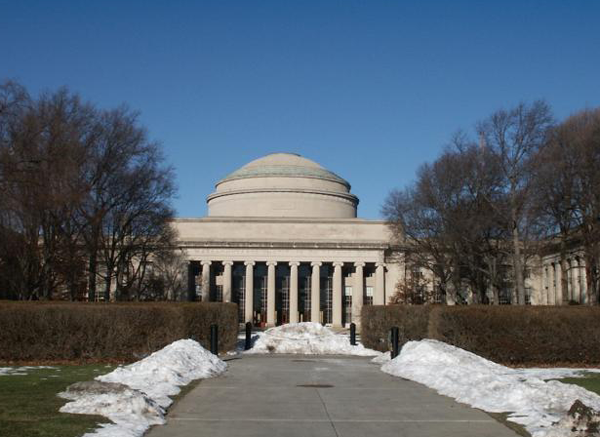
\includegraphics[width=0.9\columnwidth]{Figure1}
%\caption{With Caption Below, be sure to have a good resolution image
%  (see item D within the preparation instructions).}
%\label{fig:figure1}
%\end{figure}
%
%\subsection{References and Citations}
%
%Use a numbered list of references at the end of the article, ordered
%alphabetically by first author, and referenced by numbers in brackets
%\cite{ethics,
%  Klemmer:2002:WSC:503376.503378,
%  Mather:2000:MUT,
%  Zellweger:2001:FAO:504216.504224}. For
%papers from conference proceedings, include the title of the paper and
%an abbreviated name of the conference (e.g., for Interact 2003
%proceedings, use \textit{Proc. Interact 2003}). Do not include the
%location of the conference or the exact date; do include the page
%numbers if available. See the examples of citations at the end of this
%document. Within this template file, use the \texttt{References} style
%for the text of your citation.
%
%Your references should be published materials accessible to the
%public.  Internal technical reports may be cited only if they are
%easily accessible (i.e., you provide the address for obtaining the
%report within your citation) and may be obtained by any reader for a
%nominal fee.  Proprietary information may not be cited. Private
%communications should be acknowledged in the main text, not referenced
%(e.g., ``[Robertson, personal communication]'').
%
%\begin{table}
%  \centering
%  \begin{tabular}{|c|c|c|}
%    \hline
%    \tabhead{Objects} &
%    \multicolumn{1}{|p{0.3\columnwidth}|}{\centering\tabhead{Caption --- pre-2002}} &
%    \multicolumn{1}{|p{0.4\columnwidth}|}{\centering\tabhead{Caption --- 2003 and afterwards}} \\
%    \hline
%    Tables & Above & Below \\
%    \hline
%    Figures & Below & Below \\
%    \hline
%  \end{tabular}
%  \caption{Table captions should be placed below the table.}
%  \label{tab:table1}
%\end{table}
%
%\section{Sections}
%
%The heading of a section should be in Helvetica 9-point bold, all in
%capitals. Use Arial if Helvetica is not available. Sections should
%not be numbered.
%
%\subsection{Subsections}
%
%Headings of subsections should be in Helvetica 9-point bold with
%initial letters capitalized.  For
%sub-sections and sub-subsections, a word like \emph{the} or \emph{of}
%is not capitalized unless it is the first word of the heading.)
%
%\subsubsection{Sub-subsections}
%
%Headings for sub-subsections should be in Helvetica 9-point italic
%with initial letters capitalized.  Standard {\textbackslash}section,
%{\textbackslash}subsection, and {\textbackslash}subsubsection commands
%will work fine.
%
%\section{Figures/Captions}
%
%Place figures and tables at the top or bottom of the appropriate
%column or columns, on the same page as the relevant text
%(see Figure~\ref{fig:figure1}). A figure or table may extend across both
%columns to a maximum width of 17.78 cm (7 in.).
%
%Captions should be Times New Roman 9-point bold.  They should be numbered (e.g.,
%``Table~\ref{tab:table1}'' or ``Figure~\ref{fig:figure2}''), centered
%and placed beneath the figure or table.  Please note that the words
%``Figure'' and ``Table'' should be spelled out (e.g., ``Figure''
%rather than ``Fig.'') wherever they occur.
%
%Papers and notes may use color figures, which are included in the page
%limit; the figures must be usable when printed in black and white in
%the proceedings.  The paper may be accompanied by a short video figure
%up to five minutes in length.  However, the paper should stand on its
%own without the video figure, as the video may not be available to
%everyone who reads the paper.
%
%\section{Language, Style and Content}
%
%The written and spoken language of SIGCHI is English. Spelling and
%punctuation may use any dialect of English (e.g., British, Canadian,
%US, etc.) provided this is done consistently. Hyphenation is
%optional. To ensure suitability for an international audience, please
%pay attention to the following:
%
%\begin{itemize}
%\item Write in a straightforward style.
%\item Try to avoid long or complex sentence structures.
%\item Briefly define or explain all technical terms that may be
%  unfamiliar to readers.
%\item Explain all acronyms the first time they are used in your text---e.g.,
%``Digital Signal Processing (DSP)''.
%\item Explain local references (e.g., not everyone knows all city
%  names in a particular country).
%\item Explain ``insider'' comments. Ensure that your whole audience
%  understands any reference whose meaning you do not describe (e.g.,
%  do not assume that everyone has used a Macintosh or a particular
%  application).
%\item Explain colloquial language and puns. Understanding phrases like
%  ``red herring'' may require a local knowledge of English.  Humor and
%  irony are difficult to translate.
%\item Use unambiguous forms for culturally localized concepts, such as
%  times, dates, currencies and numbers (e.g., ``1-5-97'' or ``5/1/97''
%  may mean 5 January or 1 May, and ``seven o'clock'' may mean 7:00 am or
%  19:00).  For currencies, indicate equivalences---e.g., ``Participants
%  were paid 10,000 lire, or roughly \$5.''
%\item Be careful with the use of gender-specific pronouns (he, she)
%  and other gendered words (chairman, manpower, man-months). Use
%  inclusive language that is gender-neutral (e.g., she or he, they,
%  s/he, chair, staff, staff-hours,
%  person-years). See~\cite{Schwartz:1995:GBF} for further advice and
%  examples regarding gender and other personal attributes.
%\item If possible, use the full (extended) alphabetic character set
%  for names of persons, institutions, and places (e.g.,
%  Gr{\o}nb{\ae}k, Lafreni\'ere, S\'anchez, Universit{\"a}t,
%  Wei{\ss}enbach, Z{\"u}llighoven, \r{A}rhus, etc.).  These characters
%  are already included in most versions of Times, Helvetica, and Arial
%  fonts.
%\end{itemize}
%
%\section{Accessibility}
%The Executive Council of SIGCHI has committed to making SIGCHI conferences more inclusive for researchers, practitioners, and educators with disabilities. As a part of this goal, the all authors are asked to work on improving the accessibility of their submissions. Specifically, we encourage authors to carry out the following five steps:
%\begin{enumerate}
%	\item Add alternative text to all figures
%	\item Mark table headings
%	\item Add tags to the PDF
%	\item Verify the default language
%	\item Set the tab order to ``Use Document Structure''
%\end{enumerate}
%Unfortunately good tools do not yet exist to create tagged PDF files from Latex. LaTeX users will need to carry out all of the above steps in the PDF directly using Adobe Acrobat, after the PDF has been generated.
% 
%For more information and links to instructions and resources, please see:
%{\url{http://chi2014.acm.org/authors/guide-to-an-accessible-submission}}.
%
%\section{Page Numbering, Headers and Footers}
%Your final submission SHOULD NOT contain any footer or header string information 
%at the top or bottom of each page. The submissions will be paginated in a determined 
%order by the chairs and page numbers added to the pdf during the compiling, 
%indexing, and pagination processes.
%
%\section{Producing and Testing PDF Files}
%
%We recommend that you produce a PDF version of your submission well
%before the final deadline.  Your PDF file must be ACM DL
%Compliant. The requirements for an ACM Compliant PDF are available at:
%{\url{http://www.sheridanprinting.com/typedept/ACM-distilling-settings.htm}}.
%
%Test your PDF file by viewing or printing it with the same software we
%will use when we receive it, Adobe Acrobat Reader Version 7. This is
%widely available at no cost from~\cite{acrobat}.  Note that most
%reviewers will use a North American/European version of Acrobat
%reader, which cannot handle documents containing non-North American or
%non-European fonts (e.g. Asian fonts).  Please therefore do not use
%Asian fonts, and verify this by testing with a North American/European
%Acrobat reader (obtainable as above). Something as minor as including
%a space or punctuation character in a two-byte font can render a file
%unreadable.
%
%\section{Blind Review}
%
%For archival submissions, CHI requires a ``blind review.'' To prepare
%your submission for blind review, remove author and institutional
%identities in the title and header areas of the paper. You may also
%need to remove part or all of the Acknowledgments text.  Further
%suppression of identity in the body of the paper and references is
%left to the authors' discretion. For more details, see the submission
%guidelines and checklist for your submission category.
%
%\section{Conclusion}
%
%It is important that you write for the SIGCHI audience.  Please read
%previous years' Proceedings to understand the writing style and
%conventions that successful authors have used.  It is particularly
%important that you state clearly what you have done, not merely what
%you plan to do, and explain how your work is different from previously
%published work, i.e., what is the unique contribution that your work
%makes to the field?  Please consider what the reader will learn from
%your submission, and how they will find your work useful.  If you
%write with these questions in mind, your work is more likely to be
%successful, both in being accepted into the Conference, and in
%influencing the work of our field.
%
%\section{Acknowledgments}
%
%We thank CHI, PDC and CSCW volunteers, and all publications support
%and staff, who wrote and provided helpful comments on previous
%versions of this document.  Some of the references cited in this paper
%are included for illustrative purposes only.  \textbf{Don't forget
%to acknowledge funding sources as well}, so you don't wind up
%having to correct it later.
%
%% Balancing columns in a ref list is a bit of a pain because you
%% either use a hack like flushend or balance, or manually insert
%% a column break.  http://www.tex.ac.uk/cgi-bin/texfaq2html?label=balance
%% multicols doesn't work because we're already in two-column mode,
%% and flushend isn't awesome, so I choose balance.  See this
%% for more info: http://cs.brown.edu/system/software/latex/doc/balance.pdf
%%
%% Note that in a perfect world balance wants to be in the first
%% column of the last page.
%%
%% If balance doesn't work for you, you can remove that and
%% hard-code a column break into the bbl file right before you
%% submit:
%%
%% http://stackoverflow.com/questions/2149854/how-to-manually-equalize-columns-
%% in-an-ieee-paper-if-using-bibtex
%%
%% Or, just remove \balance and give up on balancing the last page.
%%
%\balance
%
%\section{References format}
%References must be the same font size as other body text.
%% REFERENCES FORMAT
%% References must be the same font size as other body text.

\bibliographystyle{acm-sigchi}
\bibliography{../bib/bsr,../bib/decoding,../bib/tmaillart,../bib/neurofeedback,../bib/reading_cogsci,../bib/bci,bsr,../bib/rsvp}
\end{document}
